\documentclass{standalone}
\usepackage{tikz}
\usetikzlibrary{arrows,automata,shapes,positioning,calc}

\begin{document}
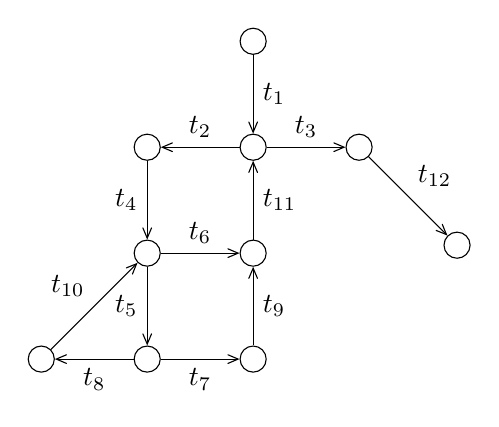
\begin{tikzpicture}
\centering
\node [circle, draw] (loc){};
\node [circle, draw] (loc1) [below=of loc]{ };
\node [circle, draw] (loc2) [left=of loc1]{ };
\node [circle, draw] (loc3) [right=of loc1]{ };
\node [circle, draw] (loc4) [below=of loc2]{ };
\node [circle, draw] (loc5) [below=of loc4]{ };
\node [circle, draw] (loc6) [right=of loc4]{ };
\node [circle, draw] (loc7) [right=of loc5]{ };
\node [circle, draw] (loc8) [left=of loc5]{ };
\node [circle, draw] (loc9) [below right=of loc3]{ };

\draw [->, -angle 45] (loc)  to node [right] {$t_1$} (loc1);
\draw [->, -angle 45] (loc1) to node [above] {$t_2$} (loc2);
\draw [->, -angle 45] (loc2) to node [left] {$t_4$} (loc4);
\draw [->, -angle 45] (loc1) to node [above] {$t_3$} (loc3);
\draw [->, -angle 45] (loc4) to node [left] {$t_5$} (loc5);
\draw [->, -angle 45] (loc5) to node [below] {$t_8$} (loc8);
\draw [->, -angle 45] (loc5) to node [below] {$t_7$} (loc7);
\draw [->, -angle 45] (loc8) to node [above left] {$t_{10}$} (loc4);
\draw [->, -angle 45] (loc7) to node [right] {$t_{9}$} (loc6);
\draw [->, -angle 45] (loc4) to node [above] {$t_6$} (loc6);
\draw [->, -angle 45] (loc6) to node [right] {$t_{11}$} (loc1);
\draw [->, -angle 45] (loc3) to node [above right] {$t_{12}$} (loc9);
\label{f:ball}
\end{tikzpicture}
\end{document}
